\documentclass[]{article}
\usepackage[spanish.mexico]{babel}
\usepackage[T1]{fontenc}
\usepackage[utf8]{inputenc}
\usepackage{lmodern}
\usepackage[a4paper]{geometry}

\usepackage{natbib}

%Grafico de barras
\usepackage{pgfplots}

%sub imagenes
\usepackage{subcaption}


%Graficos e imagenes
\usepackage{graphicx}

\title{Proyecto de Optimización de Energía}
\author{Pablo Vivar Colina}
%\date{Mayo 2018}

%%\usepackage[top=2cm,bottom=2cm,left=1cm,right=1cm]{geometry}


\begin{titlepage}
     \begin{center}
	
\includegraphics[width=0.09\textwidth]{UNAM}\Large Universidad Nacional Autónoma de México
        	
\includegraphics[width=0.09\textwidth]{FI}\\[1cm]
        \Large Facultad de Ingeniería\\[1cm]
       % \Large División de Ciencias Básicas\\[1cm]
         \Large Laboratorio de Fundamentos de Control(6655)\\[1cm]
         %la clave antes era:4314
         \footnotesize Profesor: Salcedo Ubilla María Leonor Ing.\\[1cm]
        \footnotesize Semestre 2019-1\\[1cm]
        
       

        \Large Práctica No. 1\\[1cm]
        
           

\Large Introdcción MATLAB
        
         %Texto a la derecha
          \begin{flushright}
\footnotesize  Grupo 2\\[0.5cm]
\footnotesize Brigada: 4\\[0.5cm]
\footnotesize Rodrigo Adrián Martínez López\\[0.5cm]
\footnotesize Vivar Colina Pablo\\[0.5cm]
 \end{flushright}
    %Texto a la izquierda
          \begin{flushleft}
        \footnotesize Ciudad Universitaria Agosto de 2018.\\
          \end{flushleft}
         
          
        %\vfill
        %\today
   \end{center}
\end{titlepage}
 %agregar portada

\begin{document}

\maketitle

\tableofcontents

\section{Introducción}

\subsection{Objetivo}

El siguiente proyecto tiene como objetivo ahorrar energía eléctrica en el uso doméstico en el transcurso de un semestre. Para ello, se realizará un análisis de la vivienda a optimizar realizar un plan de estrategias para practicarlas, documentarlas y hacer una comparación y revisar si las mismas han tenido efectos positivos o negativos en el consumo de energía.\\


\subsection{Conceptos}

En física, energía se define como la capacidad para realizar un trabajo. En tecnología y economía, \textit{energía} se refiere a un recurso natural (incluyendo a su tecnología asociada) para poder extraerla, transformarla y darle un uso industrial o económico.\citep{EnergiaWiki}\\

Tomando el concepto anterior nos interesa el aspecto de la energía en materia económica porque, si existe un menor consumo, por lo tanto existirá un ahorro real en capital.\\


\section{Consumo de energía Dispositivos}

\subsection{Lámpara Incandescente}

Una bombilla de incandescencia o bombilla incandescente es un dispositivo que produce luz mediante el calentamiento por efecto Joule de un filamento metálico, en concreto de wolframio, hasta ponerlo al rojo blanco, mediante el paso de corriente eléctrica. Con la tecnología existente, actualmente se considera poco eficiente, ya que el 85 $\%$ de la electricidad que consume la transforma en calor y solo el 15 $\%$ restante en luz.\citep{LamparaIncandescente}

\subsection{Lámpara fluorescente compacta}

La lámpara fluorescente compacta o lámpara fluocompacta (LFC) es un tipo de lámpara que aprovecha la tecnología de los tradicionales tubos fluorescentes para hacer lámparas de menor tamaño que puedan sustituir a las lámparas incandescentes con pocos cambios en la armadura de instalación y con menor consumo. La luminosidad emitida por un fluorescente depende de la superficie emisora, por lo que este tipo de lámparas aumentan su superficie doblando o enrollando el tubo de diferentes maneras. Otras mejoras en la tecnología fluorescente han permitido asimismo aumentar el rendimiento luminoso máximo desde los 40-50 lm/W hasta los alcanzar 80 lm/W, aunque su eficacia media actual en el mercado es de en torno a los 58 lm/W, que ha sido superado ampliamente por muchas lámparas tipo LED. También la sustitución de los antiguos electromagnéticos por balastros electrónicos ha permitido reducir el peso y el característico parpadeo de los fluorescentes tradicionales.\citep{LamparaFLuorescente}\\

En comparación con las lámparas incandescentes, las LFC tienen una vida útil más larga y consumen menos energía eléctrica para producir la misma cantidad de luz. Como desventajas, su reproducción de los colores, aunque actualmente es buena (IRC>80), no alcanza el espectro continuo de las incandescentes o halógenas (IRC=100), normalmente no alcanzan su máximo brillo de forma inmediata y es más problemático deshacerse de las viejas, pues hay que llevarlas a lugares específicos, ya que contienen residuos tóxicos. Además no es adecuado su uso en lugares cerrados pequeños o con temperatura alta, ya que se reduce drásticamente la duración por el rápido deterioro de la electrónica pudiendo llegar a explotar por sí solas bajo condiciones muy extremas.\citep{LamparaFLuorescente}\\

\subsection{Lámpara LED}

Una lámpara de ledes, también conocida como lámpara de tecnología led o más simplemente lámpara led (con led como la sigla de la tecnología de diodo emisor de luz, light emitting diode, en este caso idealmente en mayúsculas), es una lámpara de estado sólido que usa ledes (light-emitting diode, diodos emisores de luz) como fuente lumínica. Debido a que la luz capaz de emitir un led no es muy intensa, para alcanzar la intensidad luminosa similar a las otras lámparas existentes como las incandescentes o las fluorescentes compactas las lámparas led están compuestas por agrupaciones de ledes, en mayor o menor número, según la intensidad luminosa deseada.\citep{LamparaLED}

\section{Consumo hogar}

Podemos ver la instalación eléctrica de la vivienda en la figura \ref{fig:lámparas}, en ella se pueden apreciar las lámparas, contactos eléctricos y apagadores, también haremos una descripción de elementos de importancia para el análisis como lo son las ventanas.\\

 Se tiene un listado de los dispositivos que integran el funcionamiento el hogar en el cuadro \ref{tablaConsumo}. La suma de las potencias los electrodomésticos usados en el hogar es de 2250 [W].\\

\begin{figure}
    \centering
    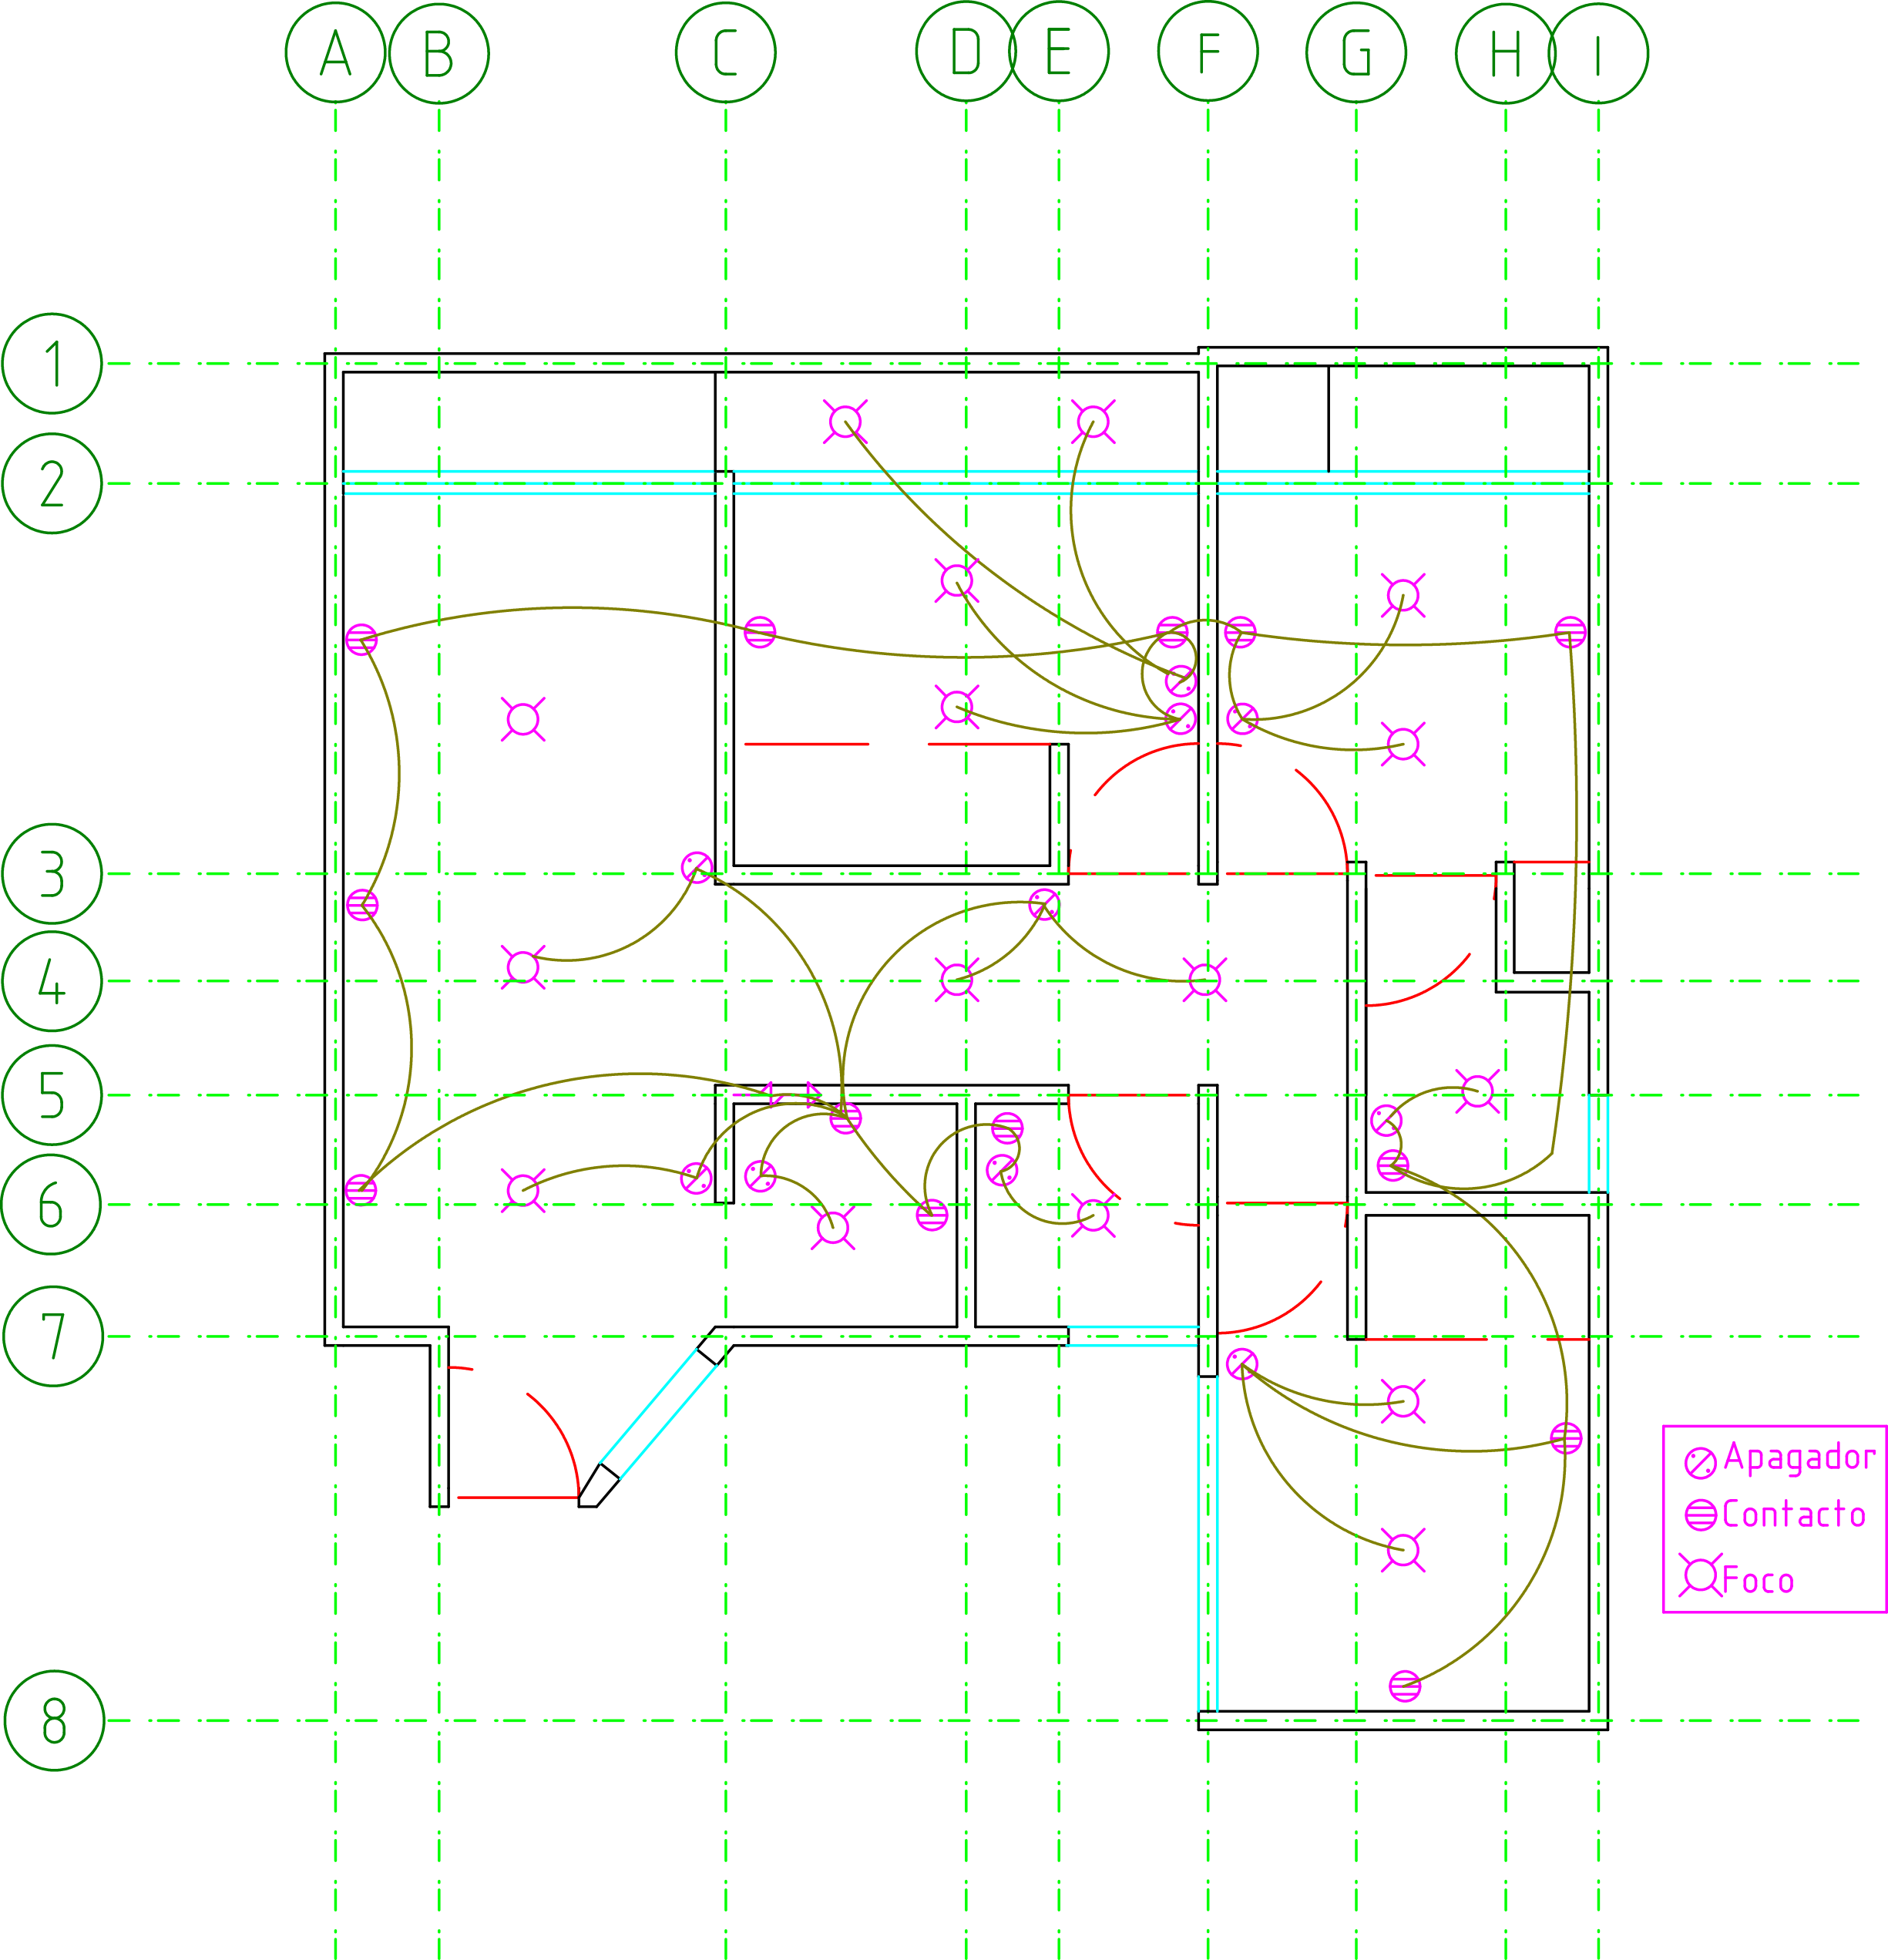
\includegraphics[width=1\textwidth]{PlanoOcaso}
    \caption{Vista de planta con conexiones eléctricas y ejes}
    \label{fig:lámparas}
\end{figure}

%Teniendo en cuenta la suma de potencias obtenidas

\begin{table}[h!]
\centering

\begin{tabular}{||c|c|c|c|c||}
\hline
Dispositivo           & Descripción                     & Cant. & Consumo {[}W{]} & Total [W] \\ \hline\hline
Lámpara Incandescente & Bombilla filamento de tungsteno & 2                  & 75              & 150           \\ \hline
Lámpara ahorradora    & Bombilla fluorescente compacta  & 10                 & 18              & 180           \\ \hline
Lámpara led           & Bombilla luz led                & 5                  & 9               & 45            \\ \hline
Microondas            & Horno de microondas             & 1                  & 1200            & 1200          \\ \hline
Refrigerador          & Aparato Refrigerador            & 1                  & 540             & 540           \\ \hline
Computadoras          & Consumo de energía aparatos     & 3                  & 25              & 75            \\ \hline
Impresoras 3D         & Energía impresión 3D            & 2                  & 30              & 60            \\ \hline
\end{tabular}
\caption{Consumo en [W] del hogar al inicio del experimento}
\label{tablaConsumo}
\end{table}

\subsection{Iluminación natural}


En cuanto Iluminación natural se refiere podemos notar en la figura \ref{fig:lámparas} que se cuentan con una buena distribución de ventanas localizadas a lo largo de eje 2, y en un tragaluz, que toca al eje F, al eje 7 y C. Esto va a ser empleado con mayor detenimiento en la sección de estrategias para el ahorro de energía como una fuente alternativa en el uso final de la energía.\\

\section{Suministro de Energía
}

En el cuadro \ref{cuadro:suministros} podemos notar el precio por [kWh] dependiendo en el rango de consumo de energía, ésta información se encuentra disponible en los recibos de energía. Y para el caso de ambos recibos comparados en éste ejercicio el rango en el cual se encuentra el consumo fué entre la escala de bajo a Intermedio, lo que dice que la vivienda tiene un buen un consumo moderado de electricidad pero que debe mejorarlo para entrar en el rango básico.\\

\begin{table}[h!]
	\centering
	\begin{tabular}[]{||c|c||}
		\hline
		 Suministro & Precio (MXN)\\
		 	\hline\hline
		 Básico & 0.820 \\
		 \hline
		 Intermedio & 0.992 \\
		 \hline
		 Excedente & 2.01 \\
		\hline
	\end{tabular}
	\caption{Suministros}
	\label{cuadro:suministros}	
\end{table}



\subsection{Historial de consumo de energía}

\begin{figure}[h!]
	\centering
	\begin{tikzpicture}
	\begin{axis}[
	symbolic x coords={A,B,C,D,E,F,G,H,I,J,K},
	xtick=data
	]
	\addplot[ybar,fill=violet] coordinates {
		(A,   284)
		(B,  291)
		(C,   274)
		(D,285)
		(E,333)
		(F,409)
		(G,437)
		(H,390)
		(I,326)
		(J,381)
		(K,331)
	};
	\end{axis}
	\end{tikzpicture}
	\caption{Consumo energía eléctrica [kWh]}
	\label{fig:grafConsumo}
\end{figure}


\begin{table}[h!]
	\centering
	\begin{tabular}[]{||c|c|c||}
		\hline
		Nombre & Periodo & Energía consumida [kWh]\\
		\hline\hline
		I & 12/Feb/19-11/Abr/19 & 326 \\
		\hline
		J & 11/Abr/19-13/Jun/19 & 381 \\
		\hline
		K & 13/Jun/19-13/Ago/19 & 331 \\
		\hline
	\end{tabular}
	\caption{Últimos periodos}
    \label{cuadro:ultimosPeriodos}
\end{table}

Según podemos ver en el cuadro \ref{cuadro:ultimosPeriodos} de los últimos periodos podemos ver que se miden cada dos meses, por lo que la energía mostrada en cada barra de la figura \ref{fig:grafConsumo} representa un periodo de 2 meses, en el cuadro \ref{cuadro:ultimosPeriodos} podemos apreciar los últimos 3 periodos de consumo de energía.\\



\section{Ahorro de energía}



\subsection{Estrategia de Cambio Focos tradicionales por LED}

De acuerdo con la sección del consumo del hogar podemos decir que se necesitan 17 bombillos, 2 de ellos incandescentes, 10 de ellos con bombilla fluorescente compacta y 5 de ellos de luz led.\\

Por lo que para un primer experimento de ahorro de energía se busca reducir la cantidad de bombillos de luz incandescente, y de luz fluorescente compacta para ser reemplazados por bombillos de luz LED preferentemente.\\

Se puede apreciar en un segundo cuadro \ref{tablaConsumoSegundo} que de los 17 focos que se necesitan en el hogar, los focos de luz incandescente han sido eliminados, y los bombillos de luz fluorescente compacta han sido reducidos, por último podemos apreciar que se aumentaron el uso de bombillos de luz LED.\\

El área que se prefiere que se intercambien por focos LED más que las demás es el área del pasillo central de la vivienda, que está localizada entre los ejes 3 a 5 y de D a F, que se puede apreciar en el plano de construcción en la figura \ref{fig:lámparas}. Porque es ésta área la que menos iluminación natural recibe, y por tanto es la que más tiene tendencia a ser encendida, si ésta parte se ilumina artificialmente al menos con tecnología LED el consumo por éste uso será menor.\\

La suma de las potencias de consumo del cuadro \ref{tablaConsumoSegundo} es de 2055 [W], comparada con la suma de potencias anteriores de 2250 [W], podemos notar una diferencia de 205 [W].\\

\begin{table}[h!]
\centering

\begin{tabular}{|c|c|c|c|c|}
\hline
Dispositivo           & Descripción                     & Cant. & Consumo {[}W{]} & Total [W] \\ \hline
Lámpara Incandescente & Bombilla filamento de tungsteno & 0                  & 75              & 0           \\ \hline
Lámpara ahorradora    & Bombilla fluorescente compacta  & 5                 & 18              & 90           \\ \hline
Lámpara led           & Bombilla luz led                & 12                  & 9               & 90            \\ \hline
Microondas            & Horno de microondas             & 1                  & 1200            & 1200          \\ \hline
Refrigerador          & Aparato Refrigerador            & 1                  & 540             & 540           \\ \hline
Computadoras          & Consumo de energía aparatos     & 3                  & 25              & 75            \\ \hline
Impresoras 3D         & Energía impresión 3D            & 2                  & 30              & 60            \\ \hline
\end{tabular}
\caption{Consumo en [W] del hogar al final del experimento}
\label{tablaConsumoSegundo}
\end{table}

\subsection{Estrategia Iluminación como uso final}

En la figura \ref{fig:lámparas} podemos apreciar la construcción de la vivienda, en ella podemos notar los cuartos que la conforman y también podemos localizar las ventanas.\\

Los cuartos que tienen cercanía con el eje 2 no tienen problema de iluminación ya que todo ese eje está conformado en su totalidad por ventanas, así que es un recurso natural que debe explotarse. Podemos notar del mismo modo que la entrada de la vivienda y el cuarto que colinda con los ejes 7, 8 y F no tienen tampoco problema de iluminación.\\

En contrario el pasillo que está en los ejes 3 a 5 tiene problemas de iluminación ya que es el espacio más central de la vivienda y no colinda con ventanas ni tragaluces, pero podemos notar que el baño que está en los ejes 5 a 7 y de D a F tiene una ventana que está comunicada con un tragaluz, así que si ese baño se mantiene con la puerta abierta y las cortinas abiertas tendremos una fuente de iluminación natural y sin tener que usar los focos de ese pasillo, que son los más recurrentes.\\

\section{Discusión}


Se puede apreciar que del periodo I al periodo J existió un aumento  de 49 [kWh], ésto probablemente causa de utilización de horas extras sobre la impresión 3D, pero en cambio para el periodo de J a K que fué en el cual se aplicaron las medidas de ahorro , el consumo descendión 44 [kWh]. Pero si se revisa el historial anterior se puede apreciar que dentro de los bimestres anteriores el consumo de energía se encuentra del rango de los niveles más bajos de energía.\\

\section{Conclusión}

Las medidas aplicadas en el experimento fueron exitosas ya que se puede apreciar una disminución en el consumo de la energía, pero es importante tener en cuenta los usos finales para poder hacer propuestas de tecnologías o medios de satisfacción de usos finales para hacer una sustitución eficiente y que se pueda apreciar un impacto sobre el consumo.\\

Como podemos notar en la figura \ref{fig:recibos} Existió un ahorro de 53 MXN debido al ahorro de consumo de energía eléctrica, y representa el $11\%$ de la energía consumida en el periodo anterior. Se necesita reestructurar las estrategias de ahorro para lograr superar éste porcentaje en los futuros bimestres y evitar que el consumo de energía vuelva a aumentar.\\

\begin{figure}[h!]
	\centering
	\begin{subfigure}[b]{0.45\textwidth}
		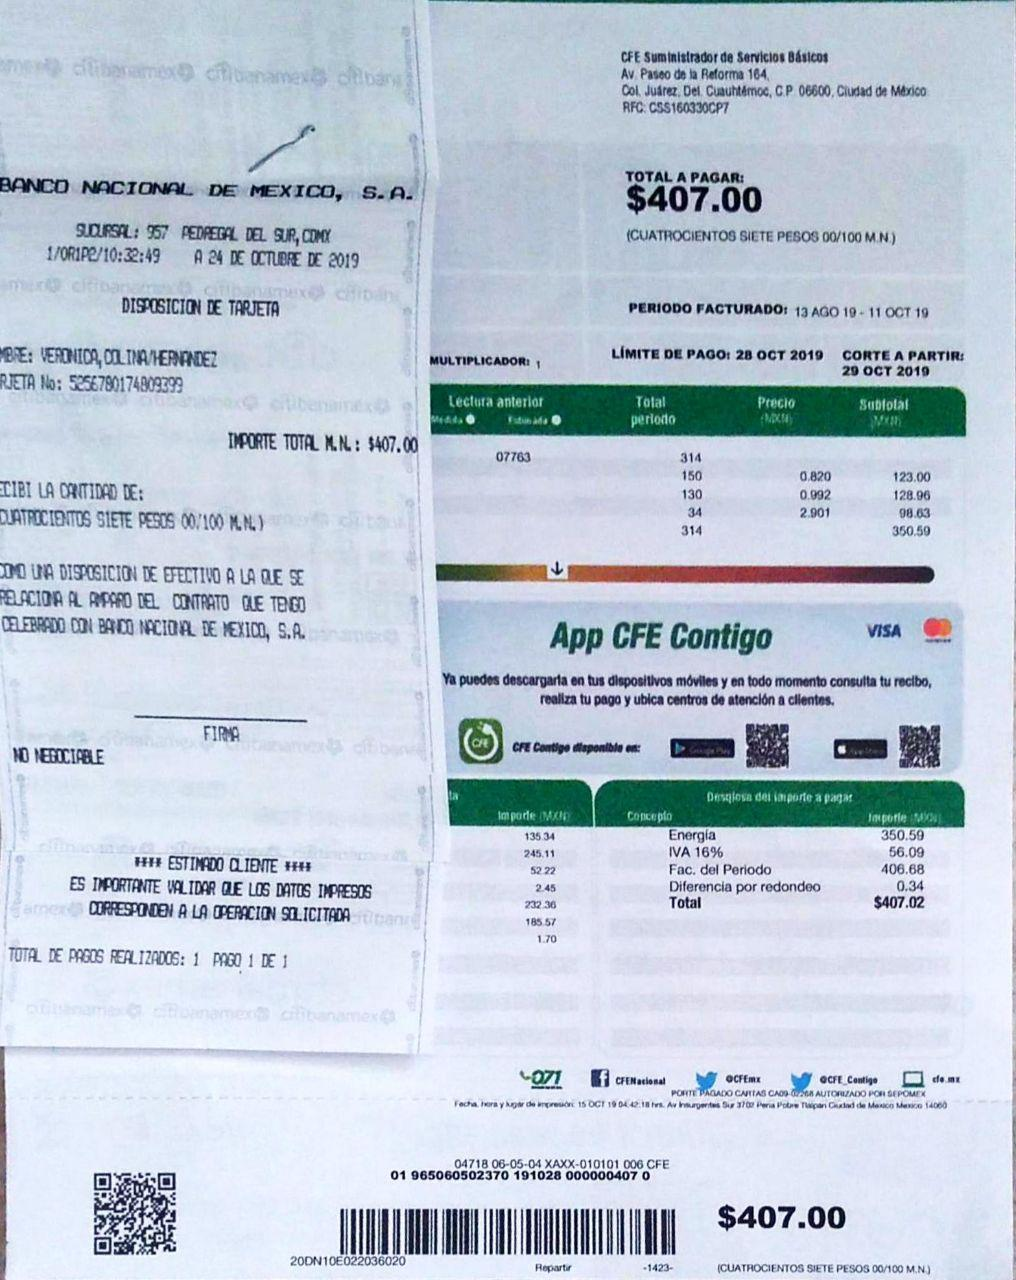
\includegraphics[width=\textwidth]{CFE1}
		\caption{Primer Recibo}
		\label{fig:CFE1}
	\end{subfigure}
	~ %add desired spacing between images, e. g. ~, \quad, \qquad, \hfill etc. 
	%(or a blank line to force the subfigure onto a new line)
	\begin{subfigure}[b]{0.45\textwidth}
		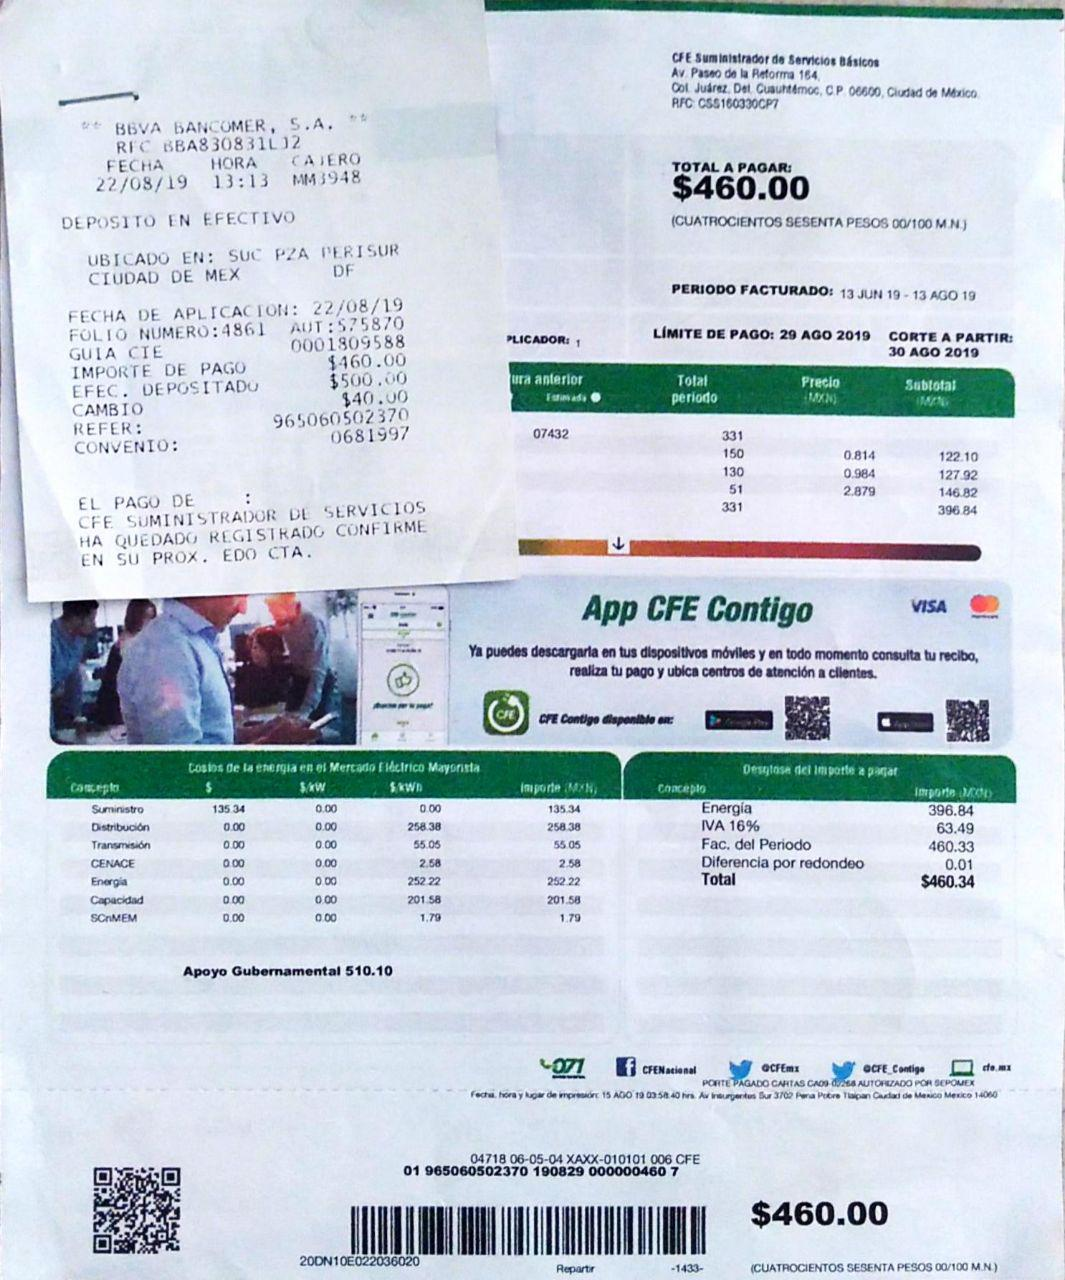
\includegraphics[width=\textwidth]{CFE2}
		\caption{Segundo Recibo}
		\label{fig:CFE2}
	\end{subfigure}
	\caption{Recibos CFE}\label{fig:recibos}
\end{figure}

%\section{GitLab}

%Quiero probando hacer cambios en gitlab.\\


\bibliographystyle{plain}
\bibliography{Referencias.bib}
%\addbibresource{Referencias.bib}
%\begin{thebibliography}{widestlabel}
%	\bibitem{EnergiaWiki}\textsc{Wikipedia}\textsc{Energia},\textit{},WikimediaGroup.
		
%\end{thebibliography}

\end{document}
